\section{Chemical geometry and illustrative structures}\label{app:chemical-geometry}
We evaluate a geometric subset of PoseBusters 0.4.4 \citep{buttenschoen2024posebusters}: heavy-atom bond lengths and angles, internal steric distances, aromatic-ring and double-bond planarity, and saturated six-membered-ring nonplanarity. The molecule-configuration tolerances are 25\% for bond and angle bounds, 30\% for internal distances, 0.25\,\AA\ for planar groups, and 0.05\,\AA\ for nonplanar rings. Accepted structures must also have zero assigned radical electrons. Conformer-ensemble energy ratios and reference-identity comparisons are excluded.

Table~\ref{tab:chemical-geometry} reports this screen and its conjunction with the 5 eV/\AA\ GFN2 force threshold. Coordinates and inferred graphs are unchanged from the original benchmark, and all 5,120 attempts per setting remain in the denominator, including inference failures.

\begin{table}[htbp]\centering\small
\caption{Geometric evaluation across five fits, with 5,120 attempts per row. ``Geometry'' requires graph validity, zero assigned radicals, and the specified local geometry checks.}
\begin{tabular}{lrrr}\toprule
Method & Graph validity & Geometry & Geometry + force\\\midrule
FM parent &20.12&3.48&1.64\\
Initial FM + physics &24.86&4.61&4.43\\
GAGA parent &22.60&4.71&2.40\\
GAGA + physics &26.25&6.64&6.45\\
LatentSpring &35.49&9.65&9.63\\
\bottomrule\end{tabular}\label{tab:chemical-geometry}
\end{table}

For the initial FM, physical correction reduces contact-disconnected outputs from 3,092 to 2,702, heavy-atom-disconnected outputs from 2,527 to 2,325, and severe overlaps from 126 to nine. Of the 1,273 graph-valid corrected outputs, 674 fail planarity, 340 fail angles, 237 fail bond lengths, and 296 fail internal distances; these categories overlap. In comparison, 470 of the 512 prepared validation references pass the same screen. Connectivity and local geometry therefore remain substantial sources of error after force correction.

\paragraph{Charge assignment.}
Among the 494 geometry-passing LatentSpring outputs on the main panel, 466 have assigned formal charges and 378 have charged carbon atoms. The corresponding counts for the 64 panel reference graphs are eight and two. Some functional groups legitimately carry formal charges, but the prevalence of these patterns in generated outputs motivates closer examination of connectivity and charge assignment. We report charge filters as separate descriptive diagnostics rather than incorporate them into the geometric criterion.

\paragraph{Common-element organic panel.}
We select validation references with 17--28 atoms, elements in CHONF, zero assigned formal charges, and passing geometric checks. Excluding the 24 development and four earlier illustration compositions leaves 13 eligible compositions. A fixed hash order selects the first 12 before generation. They are absent from the 20,000 training rows but belong to the existing validation corpus, defining a selected application-domain panel.

Each of five unchanged methods generates 16 outputs per composition from two fits: 384 attempts per method and 1,920 total. LatentSpring produces 136 geometry-and-force successes, compared with 79 for initial force-corrected FM, 68 for GAGA, 57 for EDM, and 63 for Gaussian FM. The improvement over initial FM is 14.84 points (crossed fit/composition interval $[7.81,25.52]$).

\begin{figure}[!htbp]\centering
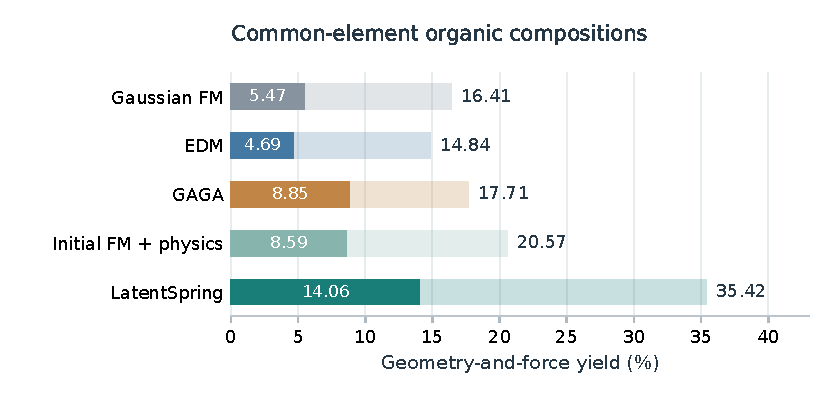
\includegraphics[width=\linewidth]{../research/figures/final_complete_v1/figures/organic_geometry.pdf}
\caption{Raw generation on 12 common-element organic compositions. Full bars show geometry-and-force yield; dark portions also require zero assigned atomic charges. Rates use all 384 attempts per method.}
\label{fig:organic-geometry}\end{figure}

Adding a zero-formal-charge filter leaves 54 LatentSpring successes and 33 initial-FM successes, or 14.06\% and 8.59\% of attempts. Excluding charged carbon gives 20.31\% and 13.02\%. These filters also exclude some reasonable ionic or charge-separated groups, so they supplement rather than replace the reported criteria.

\paragraph{Illustrated molecule.}
Figure~\ref{fig:method} shows the first full-model output in fit/composition/draw order that passes geometry and force checks with zero assigned atomic charges: fit 1, composition 1, draw 1, using one-based indices. Its formula is $\mathrm{C_7H_{15}N}$, its inferred connectivity is \texttt{CCC(C)CC=NC}, and its reported GFN2 force RMS is 1.856 eV/\AA. It is a raw output from the application panel.

The source is replayed from the original random numbers and rendered with the stored output at the same camera and scale. A PyMOL round-trip check verifies atom identities, bond orders, and coordinate precision. Figure preparation leaves the generated geometry unchanged.
